\chapter{Tema 1: Combinatoria y Teoría Elemental de Grafos}

% Permutaciones Variaciones y Combinaciones

\section{Definiciones}

\begin{definicion}
    Una \textbf{permutación} de un conjunto $X$ es una aplicación biyectiva $f:X\to X$.\\

    El conjunto de todas las permutaciones de un conjunto X se denota $Perm(X)$. En particular, si $X = \{1,2,\dots,n\}$ el conjunto de permutaciones se representa por $S_n$ y su cardinal es $n!$. (importa el orden)
\end{definicion}

\begin{definicion}
    Se llaman \textbf{variaciones sin repetición} de $n$ elementos, tomados de $m$ en $m$ a cada una de las posibles elecciones ordenadas de $m$ elementos distintos, dentro de un conjunto de $n$ elementos. (también importa el orden)
    \begin{align*}
        V_n^m = \frac{n!}{(n-m)!}
    \end{align*}
\end{definicion}

\begin{definicion}
    Se llaman variaciones con repetición de $n$ elementos, tomados de $m$ en $m$ ...
\end{definicion}

En ambos casos, dos posibles elecciones se diferencian, bien en la naturaleza de los elementos elegidos, bien en el orden en el que se han elegido.

\begin{definicion}
    Una combinación sin repetición de $n$ elementos tomados de $m$ en $m$, con $1\leq m \leq n$, es cada uno de los posibles subjconjuntos de $m$ elementos distintos dentro de un conjunto de $n$ elementos. (no importa el orden).
\end{definicion}

El número de combinaciones sin repetición de $n$ elementos tomados de $m$ a $m$, 

\begin{definicion}
    Una combinación con repetición de $n$ elementos tomados de $m$ a $m$, $1\leq m \leq n$,  es cada una de las posibles agrupaciones de $m$ elementos (no necesariamente distintos).
\end{definicion}

En ambos casos se tiene por tanto que dos combinaciones son iguales si y solo si tienen los mismos elementos sin importar el orden.

\begin{prop}
    
\end{prop}

\begin{definicion}
    Dado $\{a_1,a_2,\dots,a_m\}\subset \{1,2,\dots,n\}$, un ciclo de longitud $m$ es una permutación $\sigma \in S_n$ tal que
    \begin{align*}
        \left\{
        \begin{array}{ll}
            \sigma(a_i)= a_{i+1} & i=1,\dots,a_{m-1}\\
            \sigma(a_m)=a_1\\
            \sigma(a_j)=a_j & \forall a_j \notin\{a_1,a_2,\dots,a_m\}
        \end{array}
        \right.
    \end{align*}
    y lo representamos $\sigma = (a_1,a_2,\dots,a_m)$, pero también por $(a_2,\dots,a_m,a_1) = (a_3,\dots,a_1,a_2) = \dots = (a_m,a_1,\dots,a_{m-1})$. Hay $m$ formas distintas de representar un ciclo de longitud $m$.
\end{definicion}

\begin{ejemplo}\
    En $S_3$, los ciclos de longitud 2 son $(12), (13), (23)$ y los de longitud 3 son $(123), (231), (312); (132), (321), (213)$. El número de ciclos de longitud 3, como importa el orden, hay $V_3^3 = P_3$, pero cada ciclo de longitud 3 se expresa de 3 maneras distintas, el número de ciclos es $\dfrac{V_3^3}{3} = 2$.

    En general, el número de ciclos de longitud $m$ en $S_n = \dfrac{V_n^m}{m} $%$=\dbinom{m}{n}$ (revisar)
\end{ejemplo}

\section{Grafos. Introducción}

\begin{definicion}
    Un grafo $G$ es un par $(V,E)$, donde $V$ y $E$ son dos conjuntos, junto con una aplicación $\gamma_G:E \to \{\{u,v\} : u,v\in V\}$. $V$ es el conjunto de vértices, $E$ el conjunto de lados o aristas y $\gamma_G$ aplicación de incidencia.
\end{definicion}

\begin{ejemplo}
    Puentes de Konigsberg
\end{ejemplo}

\begin{definicion}
    Un grafo dirigido u orientado es un par $(V,E)$, donde $V$ y $E$ son conjuntos, junto con dos aplicaciones $s,t:E \to V$.
\end{definicion}

\begin{definicion}
    Sea $G=(V,E)$ un grafo con aplicación de incidencia $\gamma_G$. Un subgrafo de $G$ es un nuevo grafo $G'=(V',E')$ donde $V'\subseteq V$, $E'\subseteq E$ y se verifica que $\gamma_{G'}(e) = \gamma_G(e)$ para cualquier $e\in E'$.
\end{definicion}

\begin{definicion}
    Un subgrafo $G'$ se dice pleno si se verifica que $e\in E$ es tal que $\gamma(e)\subseteq(V')$ entonces $e \in E'$, es decir, si tiene todas las aristas de $G$ que unen vértices de $V'$.
\end{definicion}

\begin{definicion}
    Un camino es una sucesión finita de lados con la propiedad de que cada lado acaba donde empieza el siguiente.\\

    Un camino de longitud $n$ es una sucesión de lados $e_1,e_2,\dots,e_n$, junto con una sucesión de vértices $v_0,v_1,\dots,v_n$ tales que $\gamma_G(e_i) = \{v_{i-1}, v_i\}$.\\

    Un camino puede ser:
    \begin{itemize}
        \item \textbf{Cerrado:} camino que empieza y acaba en el mismo vértice.
        \item \textbf{Recorrido:} camino sin lados repetidos.
        \item \textbf{Simple:}
    \end{itemize}
\end{definicion}

Sea $G$ un grafo, si existe un camino de $u$ a $v$, entonces existe un camino simple de $u$ a $v$.\\

Sea $G$ un frafo y sean $u$ y $v$ dos vértices distintos. Si existen dos caminos simples distintos de $u$ a $v$, entonces hay un ciclo en $G$.\\

En el conjunto de vértices de un frafo $G$ se puede establecer la siguiente relación binaria $R$ (que es de equivalencia)

\begin{align*}
    u,v\in V, uRv \sii \text{existe un camino de $u$ a $v$}
\end{align*}

\begin{definicion}
    Un grafo se dice conexo si todo par de vértices están relacionados por la relación anterior, es decir, están conectados por un camino. El conjunto cociente $V/R$ es unitario.
\end{definicion}

\begin{definicion}
    Sea $G$ un grafo cuyo conjunto de vértices es $V=\{v_1,v_2,\dots,v_n\}$. Se define su matriz de adyacencia como la matriz $A\in M_n(\bb{N})$ cuyo coeficiente $a_{ij}$ es el número de aristas que unen $v_i$ con $v_j$.
\end{definicion}

\begin{propiedades}
    Para un grafo sin lazos y no dirigido se verifica que:
    \begin{itemize}
        \item los elementos de la diagonal principal son todos 0
        \item es simétrica
        \item la matriz de adyacencia no es única, depende de la ordenación de los vértices (se pasa de una a otra mediante una permutación, matriz invertuble con un 1 por fila y los demás ceros)
        \item toda matriz cuadrada con coeficientes en $\bb{N}$ es la matriz de adyacencia de algún grafo
        \item %TODO
    \end{itemize}
\end{propiedades}

\begin{teo}
    Sea $G$ un grafo y $A$ su matriz de adyacencia. En la posición $ij$ de la matriz $A^k$ aparece el número de caminos de longitud $k$ que unen $v_i$ y $v_j$.\\

    Se demuestra por inducción sobre $n$.
\end{teo}

\begin{definicion}
    Sea $G$ un grafo cuyo conjunto de vértices es $V=\{v_1,v_2,\dots,v_n\}$. Se define su \textbf{matriz de incidencia} como la matriz $A\in M_{n\times m}(\bb{N})$ cuyo coeficiente $a_{ij}$ vale $1$ si $v_i\in \gamma_G(e_j)$ y $0$ en otro caso. 
\end{definicion}

\begin{propiedades}\
    \begin{itemize}
        \item La matriz de incidencia no es única, depende de la ordenación de los vértices.
        \item Si un grafo tiene lados paralelos %TODO
    \end{itemize}
\end{propiedades}

\begin{ejemplo}
    Supongamos que tenemos la siguiente matriz de adyacencia:
    \begin{align*}
        \begin{pmatrix}
            0 & 1 & 0 & 1 & 1\\
            1 & 0 & 1 & 1 & 1\\
            0 & 1 & 0 & 0 & 0\\
            1 & 1 & 0 & 0 & 0\\
            1 & 1 & 0 & 0 & 0\\
        \end{pmatrix}
    \end{align*}
    Entonces el grafo asociado será: 
    %TODO

\end{ejemplo}

\begin{ejemplo}
    Supongamos que tenemos la siguiente matriz de adyacencia:
    \begin{align*}
        \begin{pmatrix}
            0 & 1 & 1 & 1 \\
            1 & 0 & 0 & 0 \\
            1 & 0 & 0 & 1 \\
            1 & 0 & 1 & 0 \\
        \end{pmatrix}
    \end{align*}
    Entonces el grafo asociado será: 
    %TODO
    \begin{center}
        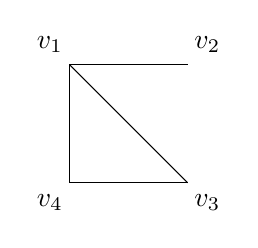
\begin{tikzpicture}
            \node at (0,0) {$v_4$};
            \node at (2,0) {$v_3$};
            \node at (0,2) {$v_1$};
            \node at (2,2) {$v_2$};

            \draw (0.25, 0.25) -- (1.75, 0.25);
            \draw (0.25, 0.25) -- (0.25, 1.75);
            \draw (0.25, 1.75) -- (1.75, 1.75);
            \draw (0.25, 1.75) -- (1.75, 0.25);
        \end{tikzpicture}
    \end{center}

\end{ejemplo}

\begin{definicion}
    Dos grafos $G$ y $G'$ se dice que son isomorfos si existen dos biyecciones $h_V:V\to V'$, $h_E: E \to E'$ tales que para cada lado $e\in E$ se verifica que $\gamma_G'(h_E(e)) = \{\}$
\end{definicion}

\begin{definicion}
    Una propiedad se dice invariante por isomorfismo si dados dos grafos isomorfos $G$ y $G'$, uno satisface la propiedad si y solo si lo satisface el otro. Los dos primeros invariantes son el número de vértices y el número de lados.
\end{definicion}

\begin{definicion}
    Sea $G$ un grafo y $v$ un vértice de $G$ se define el grado de $v$, y lo denotaremos por $gr(v)$, como el número de lados que son incidentes en $v$. Denotaremos mediante $D_k(G)$ al número de vértices de $V$ de grado $k$. A la sucesión $D_0(G), D_1(G),\dots,D_k(G),\dots$ la llamaremos sucesión de grados del grafo.
\end{definicion}

\begin{observacion}
    El grado de un vértice es un invariante por isomorfismos, esto es, $gr(v)=gr(h_V(v))$.
\end{observacion}

\begin{observacion}
    Las sucesiones de grados de dos grafos isomorfos son iguales.
\end{observacion}

\begin{propiedades}\
    \begin{itemize}
        \item La relación entre grados y lados la podemos expresar como
        \begin{align*}
            \sum\limits_i gr(v_i) = 2 \cdot l
        \end{align*}
        con $l=|E|$ el número de lados.
    
        \item En un grafo, el número de vértices de grado impar es par.
    \end{itemize}
\end{propiedades}

\begin{definicion}
    Un grafo se dice que es regular si todos los vértices tienen el mismo grado.
\end{definicion}

\begin{ejercicio}(Ejercicio 5 de la relación)\
    \begin{center}
        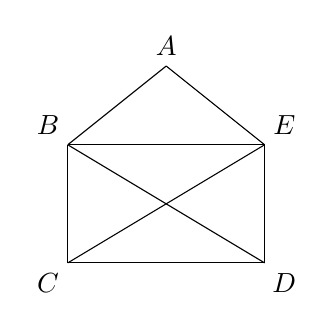
\begin{tikzpicture}
            \node at (1.5,3) {$A$};
            \node at (0,0) {$C$};
            \node at (3,0) {$D$};
            \node at (0,2) {$B$};
            \node at (3,2) {$E$};

            \draw (0.25, 0.25) -- (2.75, 0.25);
            \draw (0.25, 0.25) -- (0.25, 1.75);
            \draw (0.25, 1.75) -- (2.75, 1.75);
            \draw (0.25, 1.75) -- (2.75, 0.25);
            \draw (2.75, 1.75) -- (2.75, 0.25);
            \draw (0.25, 1.75) -- (2.75, 1.75);
            \draw (2.75, 1.75) -- (1.5, 2.75);
            \draw (0.25, 0.25) -- (2.75, 1.75);
            \draw (0.25, 1.75) -- (1.5, 2.75);
        \end{tikzpicture}
    \end{center}
\end{ejercicio} 

\begin{definicion}
    Se llama grafo completo de $n$ vértices y se denota $K_n$ al grafo (con $n$ vértices) que no tiene lados paralelos, y dados dos vértices hay un lado que los une. $|V|=n$; $|E| = \dfrac{1}{2}(n-1) \cdot n$.\\

    Su matriz de adyacencia vale $0$ en la diagonal principal y $1$ en el resto (de forma que haya $n-1$ unos en cada fila).
\end{definicion}

\begin{definicion}
    Sea $G=(V,E)$ un grafo. Se dice que $G$ es bipartido si podemos descomponer $V$ en dos subconjuntos disjuntos $V_1$ y $V2$ de manera que todo lado incide en un vértice de $V_1$ y en un vértice de $V_2$. $|V| = |V_1| + |V_2|$.
\end{definicion}

\begin{definicion}
    Un grafo $G=(V,E)$ se dice bipartido completo si es bipartido y para cada $v_1\in V_1$ y $v_2\in V_2$ existe un único lado $e\in E$ tal que $\gamma(e)=\{v_1,v_2\}$. Se denotan mediante $K_{n,m}$, donde $n=|V_1|$ y $m=|V_2|$. En este cado, $|V| = m + n $ y $|E| = m \cdot n$.
\end{definicion}

\begin{definicion}
    Un grafo $G=(V,E)$ se dice ciclo con $n$ vértices si cada vértice es incidente únicamente con los vértices anterior y posterior. $|V|=n$ y $|E|=n$. Se denota mediante $C_n$.
\end{definicion}

\begin{definicion}
    Un grafo $G=(V,E)$ se dice rueda con $n$ vértices si cada vértice es incidente únicamente con los vértices anterior y posterior y con un tercer vértice central. $|V| = n+1$ y $|E|=2n$. Se denota mediante $W_n$.
\end{definicion}

\begin{definicion}
    Sean $d_1,d_2,\dots,d_n\in \bb{N}$. Decimos que la sucesión $d_1,d_2,\dots,d_n$ es una sucesión gráfica si existe un grafo $G$ sin lazos, ni lados paralelos con $n$ vértices $\{v_1,v_2,\dots,v_n\}$ y tal que $gr(v_i)=d_i$. Diremos que $G$ es una realización de la sucesión $d_1,d_2,\dots,d_n$.
\end{definicion}

\begin{teo}(Havel-Hakini)\ 
    
    Sea $d_1,d_2,\dots,d_n$ una sucesión de números naturales ordenada $(d_1 \geq d_2 \geq \dots \geq d_n)$ y con $d_1 < n$. Entonces $d_1,d_2,\dots,d_n$ es una sucesión gráfica si y solo si $d_2-1, d_3-1,\dots,d_{d_1+1}-1,d_{d_1+2},\dots,d_n$ es una sucesión gráfica.
\end{teo}

\begin{definicion}
    Un camino de Euler en un grafo G es un recorrido en el que aparecen todos los lados.
\end{definicion}

\begin{definicion}
    Un circuito de Euler es un camino de Euler cerrado .
\end{definicion}

\begin{definicion}
    Un grafo G es un grafo de Euler si es conexo y tiene un circuito de Euler.
\end{definicion}

\begin{teo}
    Un grafo conexo es de Euler si y solo si todos sus vértices son de grado par.
    \begin{proof}\
        \begin{itemize}
            \item[$\Rightarrow$)] Supongamos que $G$ es conexo y es de Euler. Sea $\alpha$ un circuito de Euler y para cada vez que pasamos por un vértice le estamos añadiendo un grado 2 al vértice. Como cada lado aparece una sola vez, entonces el grado es múltiplo de 2.
            \item[$\Leftarrow$)] Se hace por inducción. Veamos qué ocurre para el caso $n=4$. Hagamos la siguiente partición:% PEDIR DIBUJO TODO A ALI
            \begin{align*}
                \sigma_1 = v_1 e_1 v_2 e_2 v_3 e_6 v_1\\
                \sigma_2 = v_3 e_3 v_4 e_4 v_5 e_1 v_3\\
                \sigma_3 = v_2 e_9 v_4 e_{10} v_1 e_3 v_3 v_2\\
            \end{align*}
            y hacemos el siguiente circuito, conectando los anteriores por $v_3$ y $v_4$:
            \begin{align*}
                \sigma = v_3 e_6 v_1 e_1 v_2 e_2 v_3 e_3 v_4 e_{10} v_1 e_5 v_5 e_8 v_2 e_9 v_4 e_4 v_5 e_7 v_3
            \end{align*}
        \end{itemize}
    \end{proof}
\end{teo}

